\documentclass[10pt]{beamer}
\usetheme{Madrid}
\usecolortheme{default}
\usepackage{amsmath,amssymb}
\usepackage{tikz}
\usepackage{booktabs}

\newcommand{\PP}{\mathcal{P}}
\newcommand{\qpoch}[2]{(#1;#2)}

\title[Euler's Pentagonal Number Theorem]{Euler's Pentagonal Number Theorem}
\subtitle{Formalization via Franklin's involution \,\&\, the Jacobi triple product}
\author{JC, PM, MV}
\date{\today}

\begin{document}

\frame{\titlepage}

% ======================================================================
\section{Euler's Pentagonal Number Theorem}
% ======================================================================

\begin{frame}{The theorem}
\begin{block}{Euler's Pentagonal Number Theorem}
\[
\prod_{n=1}^{\infty}\bigl(1-x^{n}\bigr)
 \;=\; \sum_{k=-\infty}^{\infty} (-1)^{k}\, x^{\,k(3k-1)/2}
 \;=\; 1+\sum_{k=1}^{\infty}(-1)^{k}\Bigl(x^{\frac{k(3k-1)}2}+x^{\frac{k(3k+1)}2}\Bigr).
\]
\end{block}
\pause
\textbf{Combinatorial form.} Let $p_e(n)$ (resp.\ $p_o(n)$) count partitions of $n$
into an \emph{even} (resp.\ \emph{odd}) number of \emph{distinct} parts. Then
\[
p_e(n)-p_o(n)=
\begin{cases}
(-1)^{k} & n=\tfrac{3k^{2}\pm k}{2}\ \ (\text{pentagonal}),\\[2pt]
0 & \text{otherwise.}
\end{cases}
\]
\begin{center}
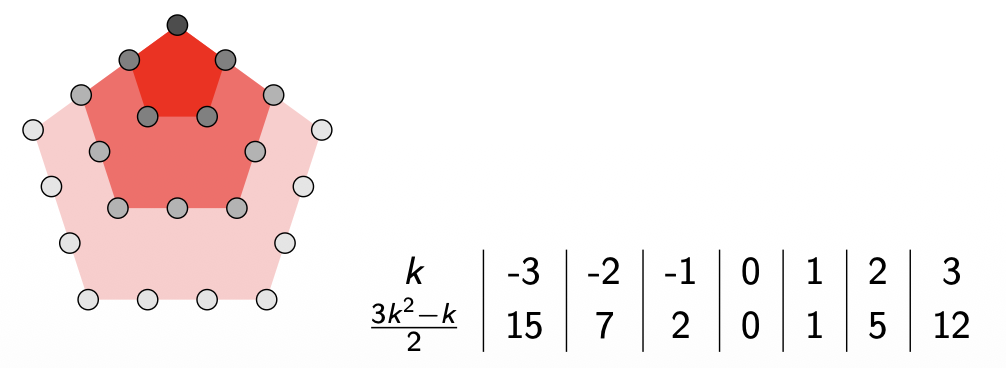
\includegraphics[width=0.56\textwidth]{PentNumbers}\\[-3pt]
{\scriptsize Generalized pentagonal numbers $\tfrac{3k^2-k}{2}$ ($k\in\mathbb Z$): $0,1,2,5,7,12,15,\dots$}
\end{center}
\end{frame}

\begin{frame}{Base, slope, and Franklin's involution}
\begin{columns}[T]
\begin{column}{0.46\textwidth}
\centering
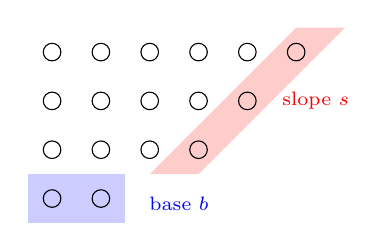
\begin{tikzpicture}[scale=0.62]
\fill[blue!20!white] (-0.5,-3.5)--(1.5,-3.5)--(1.5,-2.5)--(-0.5,-2.5);
\fill[red!20!white] (2.,-2.5)--(3.,-2.5)--(6.,0.5)--(5.,0.5);
\draw (5.4,-1) node{\scriptsize\color{red}slope $s$};
\draw (2.6,-3.1) node{\scriptsize\color{blue}base $b$};
\foreach \x in {0,...,5}{\draw (\x,0) circle(0.18cm);}
\foreach \x in {0,...,4}{\draw (\x,-1) circle(0.18cm);}
\foreach \x in {0,...,3}{\draw (\x,-2) circle(0.18cm);}
\foreach \x in {0,1}{\draw (\x,-3) circle(0.18cm);}
\end{tikzpicture}\\[2pt]
{\scriptsize Diagram of $17=6+5+4+2$.}
\end{column}
\begin{column}{0.54\textwidth}
\small
$b=\min(S)$, $m=\max(S)$,\\
$s=$ length of the top consecutive run,\\
$D=\{m-s+1,\dots,m\}$ the slope set.
\medskip

A partition lies in exactly one class:
\[
\PP(n)=\PP_\alpha(n)\sqcup\PP_\beta(n)\sqcup\PP_{\mathrm{special}}(n).
\]
\[
\alpha(S)=(S\setminus\{b,m{-}b{+}1\})\cup\{m{+}1\}
\]
\[
\beta(S)=(S\cup\{s,m{-}s\})\setminus\{m\}
\]
\end{column}
\end{columns}
\end{frame}

\begin{frame}{Proof sketch (Franklin's involution)}
Define $F=\alpha$ on $\PP_\alpha$, $\;\beta$ on $\PP_\beta$, and the identity on $\PP_{\mathrm{special}}$.
\begin{enumerate}
\item $\alpha:\PP_\alpha\to\PP_\beta$ and $\beta:\PP_\beta\to\PP_\alpha$ are mutually inverse
      $\Rightarrow$ $F$ is an \alert{involution} with $\beta\circ\alpha=\mathrm{id}$, $\alpha\circ\beta=\mathrm{id}$.
\item $F$ \alert{preserves $n$} and \alert{flips the parity} of the number of parts on $\PP_\alpha\cup\PP_\beta$.
\item Hence $\alpha,\beta$ pair off even with odd partitions: they cancel in $p_e-p_o$.
\item Only the \alert{fixed points} $\PP_{\mathrm{special}}(n)$ survive: empty unless $n$ is
      pentagonal, where it is a single staircase $\{k,\dots,2k{-}1\}$ or $\{k{+}1,\dots,2k\}$
      of parity $(-1)^k$.
\end{enumerate}
\[
\boxed{\,p_e(n)-p_o(n)=\sum_{S\in\PP_{\mathrm{special}}(n)}(-1)^{|S|}
=\begin{cases}(-1)^k & n=\tfrac{3k^2\pm k}2\\ 0&\text{else.}\end{cases}}
\]
\end{frame}

% \begin{frame}{Lean formalization (\texttt{Aristotle/}) --- $\approx$ 1{,}036 lines, \texttt{sorry}-free}
% \centering\small
% \begin{tabular}{@{}llcl@{}}
% \toprule
% Component (file) & Lemmas & Lines & Effort \\
% \midrule
% Definitions (\texttt{Defs}) & $\PP_\alpha,\PP_\beta,\PP_{\mathrm{spec}}$, base/slope & 90 & Low \\
% Helpers (\texttt{Helpers}) & run/slope, $b\le m$, $m\ge 2b$ & 322 & \alert{High -- manual induction} \\
% Disjoint + trichotomy & Lem.\ 11--12 & $\sim$26 & Low -- \texttt{grind}/\texttt{simp} \\
% Special $=$ pentagonal & Lem.\ 13--14 & $\sim$230 & Med.\ -- arithmetic \\
% Franklin involution & Lem.\ 16--19 & $\sim$120 & \alert{High -- very manual} \\
% Bijection \& counting & Lem.\ 20--24 & $\sim$135 & Med.\ -- \texttt{Finset.card} \\
% \bottomrule
% \end{tabular}
% \medskip

% \footnotesize
% \textbf{Easy:} definitions, disjointness/trichotomy (one \texttt{grind} each), final assembly.\\
% \textbf{Hard / very manual:} reasoning about \emph{slope} (a recursive top-run) and \emph{base/max}
% under $\cup/\setminus$; the four involution lemmas $\alpha\!\in\!\PP_\beta$, $\beta\!\in\!\PP_\alpha$,
% $\beta\!\circ\!\alpha=\mathrm{id}$, $\alpha\!\circ\!\beta=\mathrm{id}$.\\
% \textbf{Library-assisted:} cardinality/bijection step rides on mathlib's \texttt{Finset}.
% \end{frame}

\begin{frame}{Three formalizations of the \emph{same} bijective proof}
All three prove Euler's PNT via Franklin's involution; they differ in how much
structure is spelled out, the size of the input prompt, and whether the proof closes.
\centering\small
\begin{tabular}{@{}lccc@{}}
\toprule
 & \texttt{Aristotle} & \texttt{SlidesInput} & \texttt{OnlyWordsInput} \\
\midrule
Total lines        & \textbf{1{,}350}      & \textbf{728}        & \textbf{854} \\
Files              & 5                     & 3                   & 3 \\
Status             & \alert{\texttt{sorry}-free} & \alert{\texttt{sorry}-free} & 1 \texttt{sorry} \\
\bottomrule
\end{tabular}
\medskip

\footnotesize
\begin{itemize}
\item \textbf{\texttt{Aristotle} (1{,}350):} explicit \emph{three-class} split
      $\PP=\PP_\alpha\sqcup\PP_\beta\sqcup\PP_{\mathrm{spec}}$ with \emph{two separate}
      maps $\alpha,\beta$ proven mutually inverse, plus a \texttt{FormalPowerSeries}
      layer linking $p_e-p_o$ to $\prod(1-X^i)$. Most verbose, fully self-contained.
\item \textbf{\texttt{SlidesInput} (728):} \emph{one} map \texttt{franklinMap} (ops A/B
      via a staircase length \texttt{stairLen}); non-fixed points cancel, fixed points
      characterized as the two staircases $\{k..2k{-}1\}$, $\{k{+}1..2k\}$. Same content,
      tighter packaging.
\item \textbf{\texttt{OnlyWordsInput} (854, was 460):} word-only prompt; rides mathlib's
      \texttt{Finset.sum\_involution} and a \texttt{topRun} helper. A 2nd run discharged the
      \emph{involutivity} lemma (\texttt{franklinInv\_invol}, $+\sim$400\,ln of helpers),
      leaving \emph{one} \texttt{sorry}: the fixed-point sum $=\texttt{pentagonalCoeff}$.
\end{itemize}
\medskip
% \footnotesize\emph{Same mathematics, now a $\sim$1.85$\times$ length spread. Pushing the once-leanest
% run (OnlyWordsInput, $460\!\to\!854$ over a 2nd run) to close the involution lemma made it
% \emph{longer} than the one-shot SlidesInput (728) --- discharging \texttt{sorry}s costs lines,
% and one still remains.}
\end{frame}

% ======================================================================
\section{The Jacobi triple product route}
% ======================================================================

\begin{frame}{Jacobi triple product (plain form)}
\begin{block}{Jacobi triple product}
\[
\prod_{m=1}^{\infty}\bigl(1-q^{2m}\bigr)\bigl(1+q^{2m-1}w^{2}\bigr)\bigl(1+q^{2m-1}w^{-2}\bigr)
\;=\;\sum_{k=-\infty}^{\infty} q^{k^{2}}\,w^{2k}.
\]
\end{block}
Equivalently, with $z=-w^{2}$,
\[
\qpoch{q}{q}_\infty\,\qpoch{-z}{q}_\infty\,\qpoch{-q/z}{q}_\infty
\;=\;\sum_{k\in\mathbb Z} z^{k}q^{k(k-1)/2}.
\]
A single bilateral identity that specializes to many classical $q$-series results.
\end{frame}

\begin{frame}{$q$-Pochhammer symbols and the $q$-binomial theorem}
\textbf{Finite / infinite $q$-Pochhammer symbol:}
\[
\qpoch{a}{q}_n=\prod_{k=0}^{n-1}\bigl(1-a q^{k}\bigr),\qquad
\qpoch{a}{q}_\infty=\prod_{k=0}^{\infty}\bigl(1-a q^{k}\bigr).
\]
\textbf{Gaussian binomial coefficient:}
$\displaystyle \binom{n}{k}_q=\frac{\qpoch{q}{q}_n}{\qpoch{q}{q}_k\,\qpoch{q}{q}_{n-k}}$.
\medskip
\begin{block}{$q$-binomial theorem (finite, then $n\to\infty$)}
\[
\prod_{k=0}^{n-1}\bigl(1+z q^{k}\bigr)=\sum_{k=0}^{n} q^{\binom{k}{2}}\binom{n}{k}_q z^{k},
\qquad
\sum_{n\ge0}\frac{\qpoch{a}{q}_n}{\qpoch{q}{q}_n}z^{n}=\frac{\qpoch{az}{q}_\infty}{\qpoch{z}{q}_\infty}.
\]
\end{block}
\footnotesize The two Euler identities follow by $a=0$ and $a\to\infty$; the Jacobi
triple product is then a short corollary. \emph{(Lean: \texttt{qBinom\_finite\_thm},
\texttt{qBinom\_infinite\_thm} --- high up-front cost, low marginal.)}
\end{frame}

\begin{frame}{Euler's PNT from the Jacobi triple product}
Start from the Jacobi triple product
\[
\prod_{m\ge1}\bigl(1-q^{2m}\bigr)\bigl(1-q^{2m-1}z\bigr)\bigl(1-q^{2m-1}z^{-1}\bigr)
=\sum_{k\in\mathbb Z}(-1)^{k}z^{k}q^{k^{2}}.
\]
\pause
Specialize $\;q\mapsto x^{3/2},\ z\mapsto x^{1/2}$:
\[
\underbrace{\prod_{m\ge1}(1-x^{3m})(1-x^{3m-1})(1-x^{3m-2})}_{=\ \prod_{n\ge1}(1-x^{n})}
\;=\;\sum_{k\in\mathbb Z}(-1)^{k}\,x^{(3k^{2}+k)/2}.
\]
\pause
The three residue classes $\bmod\,3$ reassemble the full product $\prod_{n\ge1}(1-x^n)$,
and $(3k^{2}+k)/2$ ranges over the pentagonal numbers. Hence
\[
\boxed{\ \prod_{n\ge1}(1-x^{n})=\sum_{k\in\mathbb Z}(-1)^{k}x^{\,k(3k-1)/2}\ }
\]
--- exactly Euler's Pentagonal Number Theorem, now an analytic corollary rather than
a bijective one.
\end{frame}


% ======================================================================
\begin{frame}{Formalizing the $q$-series route: where Aristotle struggled}
\footnotesize
Unlike the Franklin-involution PNT (\textbf{one} Aristotle run each), the Jacobi
triple product took \alert{$\sim$6 documented runs} to close --- two of which produced
\emph{no code}, only cost/feasibility analyses.
\medskip

\begin{itemize}
\item \textbf{Two planned routes abandoned.}
  \emph{(i)} Complex analysis / Liouville: needs holomorphicity of infinite products and a
  Liouville theorem on $\mathbb C^\ast$ --- \alert{not in mathlib} ($\sim$900--1500 lines of new
  infrastructure). \emph{(ii)} Hermite-style coefficient recurrence ($A_{n,k}$ bookkeeping):
  $\sim$1500--2000 lines. Both judged too costly.
\item \textbf{The crux: annulus $\to$ punctured disc.} The Cauchy-product proof first only
  worked on $\|q\|<\|z\|<1$; the naive extension hit \alert{boundary cases $\|z\|=\|q\|^n$} and
  stalled at one stubborn \texttt{sorry} for a full run.
\item \textbf{Solution (Aristotle).} Prove the 2nd Euler identity for \emph{all} $z$ (not just
  $\|z\|<1$) via the series recurrence $S(z)=(1+z)\,S(qz)$ --- this \alert{removes the annulus
  restriction entirely}, and the product argument runs directly on $0<\|z\|<1$.
\item \textbf{Infrastructure-heavy core.} Cauchy product over $\mathbb N\times\mathbb N$
  (Fubini + diagonal split), each diagonal evaluated by the Durfee-rectangle identity
  $S_k=1/(q;q)_\infty$ --- proved by an \emph{analytic contraction recurrence}, not the
  textbook bijection.
\end{itemize}
\smallskip
\centering\footnotesize\emph{Trajectory: 3 \texttt{sorry}s $\to$ 1 $\to$ 0 across runs;
final $\sim$1{,}700-line \texttt{sorry}-free library --- but only after iteration and planning
the bijective proof never needed.}
\end{frame}

% ======================================================================
\begin{frame}{LLM usage}
\centering\small
\begin{tabular}{@{}lrrrr@{}}
\toprule
Model & Output & Input & Cache write & Cache read \\
\midrule
Opus 4.7    & 4.1\,M  & 61\,K   & 25\,M   & 456\,M \\
Sonnet 4.6  & 1.02\,M & 0.6\,K  & 2.76\,M & 21.4\,M \\
\midrule
\textbf{Total (interactive, est.)} & \textbf{5.1\,M} & \textbf{62\,K} & \textbf{28\,M} & \textbf{477\,M} \\
\midrule
Aristotle (\emph{est.}) & \multicolumn{4}{c}{$\approx$\,55--145\,M total --- \alert{$\sim$9--13 runs} total} \\
\bottomrule
\end{tabular}
\medskip

\footnotesize
\begin{itemize}
% \item $\approx$\,510\,M tokens total over the whole project. $\sim$94\% are \emph{cache reads}:
%       the full context (system prompt, tools, files, tool outputs, all prior turns) is
%       re-read every turn, so cache-read $\approx$ (context size) $\times$ (\#turns) --- it
%       compounds, while output is only what is generated each turn.
\item \textbf{Interactive cost @ API rates} (standard Opus/Sonnet tiers, \emph{not} the Max plan;
      recorded $+$ this session, est.): $\approx\$1{,}500$ \,(\$1{,}465 Opus $+$ \$32 Sonnet; output \$310,
      cache-read \$685, cache-write \$470), $\sim$15\,kWh compute / $\sim$19\,kWh with datacenter
      overhead --- $\approx$ driving an EV $\sim$110\,km, or a fridge for $\sim$2 weeks.
\item \textbf{Aristotle (est.\ --- no token logs; from run counts):}
      OnlyWordsInput \alert{2 runs} / 854\,ln / 1 \texttt{sorry}; SlidesInput 1 run / 728\,ln / closed;
      qSeries+JTP \alert{6 documented runs} (2 spent only on feasibility/cost analysis) / 1.7\,k\,ln / closed.
      Total $\sim$9--13 runs, $\approx$55--145\,M tok, $\approx\$220$--$880$, $\approx$4.5--22\,kWh.
% \item \emph{Energy assumptions:} $\sim$3\,J per output token, $\sim$0.5\,J per prefill
%       (input $+$ cache-write) token, $\sim$0.05\,J per cache-read token (cheap KV reuse),
%       $\times$1.3 datacenter PUE. Per-run Aristotle: $\sim$5--15\,M tok, $\sim\$20$--$80$, $\sim$0.5--2\,kWh.
\item \textbf{Summary:} Generating proofs is cheaper than talking about them.
\end{itemize}
\end{frame}

\end{document}
